%! TeX program = lualatex
\documentclass{article} 

\title{Wielomian Alexandera}
\author{Weronika Jakimowicz}
\date{}

\usepackage{tikz}
\usetikzlibrary{cd, patterns, patterns.meta, decorations.pathmorphing, calc, matrix, positioning, arrows, arrows.meta}
\usetikzlibrary{spath3, hobby, knots, braids}

\usepackage{graphicx}

\usepackage[T1]{fontenc}

\usepackage{fontspec}
\usepackage[default]{cantarell}

\usepackage[nolessnomore,noequal,noparenthesis,nospecials,noplusnominus,noexclam,italic]{mathastext}

\usepackage{amsfonts}
\usepackage{amsmath}
\usepackage{amssymb}

\usepackage{array}


\usepackage{ntheorem}

\theorembodyfont{\normalfont}
\theoremseparator{.\hspace{0.5em}}
\theorempreskip{}
\theorempostskip{}

\theorempostwork{\vspace*{4mm}}

\newtheorem{zadanie}{Zadanie}


\pagestyle{empty}

\usepackage{tikz}
\usetikzlibrary{calc}

\usepackage[a4paper, total={170mm, 237mm}]{geometry}

\usepackage{enumitem}

\newcommand{\rozwiazanie}[1]{\slshape }%#1}

\makeatletter
\def\@maketitle{
  \begin{center}
    {\LARGE\@title}
    \medskip 

    \large\@author
  \end{center}
}
\makeatother

 

\begin{document}

\maketitle 

\section{Macierze}

\section{Węzły - definicje}

\begin{definition}{Węzeł}{}
Węzeł to sposób ułożenia okręgu w przestrzeni $3$ wymiarowej tak, by dało się spojrzeć na niego z góry i w każdym punkcie zobaczyć nie więcej niż dwa punkty z okręgu. 

Tzn. nie możemy mieć $3$ sznurków z węzła przecinających się w jednym miejscu.
\end{definition}

\begin{center}
  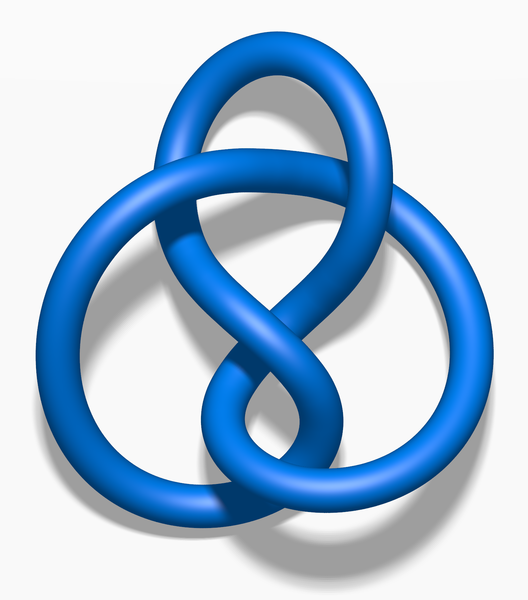
\includegraphics[width=10cm]{knot_4_1.png}

  Węzeł zwykle używany do robienia guzełków, matematycznie znany jako $4_1$, bo ma $4$ skrzyżowania.
\end{center}

Zauważmy, że ten węzeł można łatwo zmienić tak, by wyglądał na węzeł o $5$ skrzyżowaniach (na tablicy narysuję pierwszy ruch na którejś nitce). W gruncie rzeczy taki ruch nie zmienia nam węzła - jak pociągniemy za sznurówki to nadal dostaniemy guziołek z $4_1$.

Matematycznie, dwa węzły są \emph{równoważne}, czyli takie same, jeśli można jeden w drugi przekształcić za pomocą tak zwanych \textbf{ruchów Reidemeistera}.

\begin{center}
  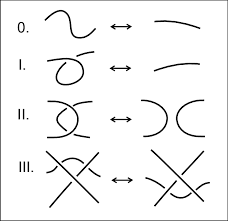
\includegraphics[width=10cm]{reidemeister_moves.png}

  Ruchy Reidemeistera, można wykonywać je w obie strony.
\end{center}

{\centering\bfseries\large\color{green!70!black}
  Pojawia się pytanie, jak szybko sprawdzić, czy dwa skomplikowane węzły są tym samym?
}

Weźmy na przykład dwa węzły jak niżej, jeden o $6$ skrzyżowaniach, a drugi o $9$.

\begin{center}
  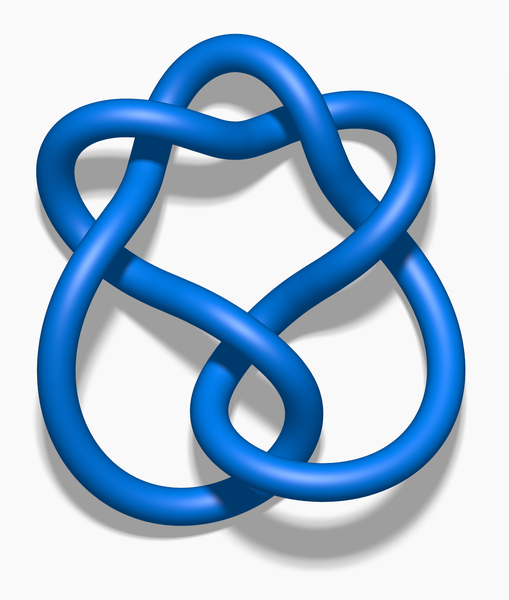
\includegraphics[width=8cm]{knot_6_1.png}
  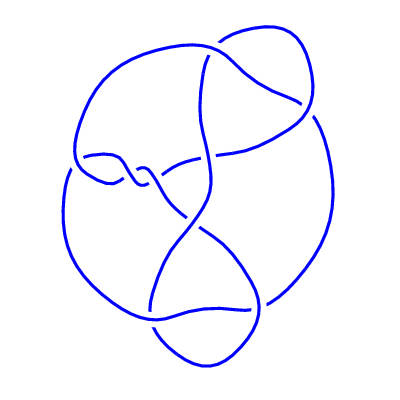
\includegraphics[width=8cm]{knot_9_46.png}

  Po lewej jest węzeł $6_1$ a po prawej $9_{46}$.
\end{center}

\section{Orientacja węzła i diagramu}

Na okręgu możemy narysować strzałkę. Ta strzałka jest zachowywana, gdy robimy z okręgu węzeł.

\begin{definition}{Zorientowany węzeł}{}
  Węzeł z zaznaczoną strzałką nazwiemy węzłem zorientowanym.
\end{definition}

W zorientowanym diagramie zawsze mamy dwa rodzaje skrzyżowań:
\begin{center}
  \begin{tikzpicture}
    \draw[->, very thick] (0, 0)--(0, 3);
    \fill[white] (0, 1.5) circle (5pt);
    \draw[->, very thick] (-1.5, 1.5)--(1.5, 1.5);

    \node at (0, -.5) {\Large\bfseries+};


    \draw[->, very thick] (4.5, 0)--(4.5, 3);
    \fill[white] (4.5, 1.5) circle (5pt);
    \draw[<-, very thick] (3, 1.5)--(6, 1.5);

    \node at (4.5, -.5) {\Large\bfseries-};
  \end{tikzpicture}
\end{center}
Nazwiemy je $+$ i $-$ tak jak na obrazku. Które skrzyżowanie jest $+$ nie ma znaczenia - ważne jest aby trzymać się cały czas jednej konwencji.

W zorientowanych diagramach węzłów mamy o jeden ruch Reidemeistera więcej. Ruch 1 z obrazka wyżej musi mieć dwa warianty - dla skrzyżowania $+$ i dla skrzyżowania $-$.

\begin{center}
  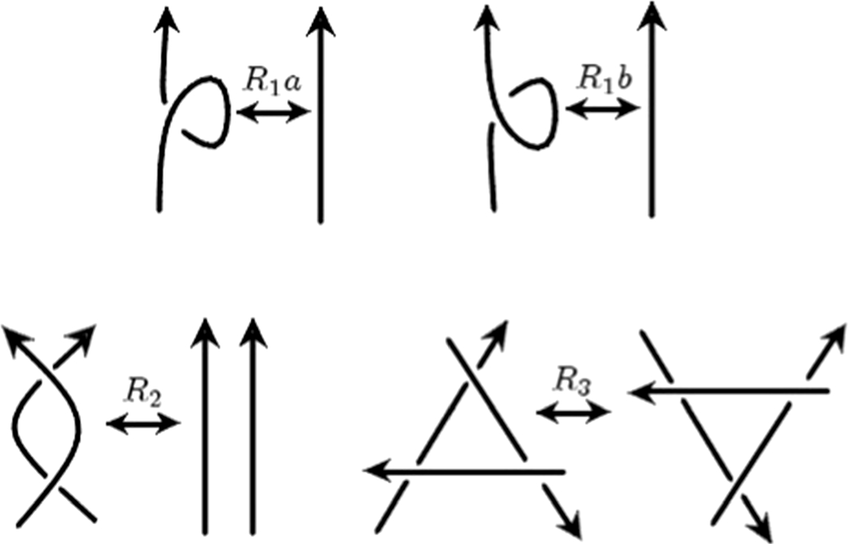
\includegraphics[width=10cm]{oriented_reidemeister.png}
\end{center}

Zdarza się, że jedna orientacja węzła nie jest równoważna przeciwnej orientacji tego samego węzła. To nas jednak nie interesuje, bo niezmiennik węzła, jakim się dzisiaj zajmiemy rozróżnia węzły, a nie ich orientacje. Istnieją inne niezmienniki, które jednak zwracają na to uwagę, np. wielomian Jonesa.

\section{Kolorowanie węzłów}

Ściśle rzecz biorąc, węzłów nigdy nie kolorujemy - robimy to z ich diagramami. W diagramach zawsze skrzyżowania będą nam mówić, czy kolorowanie jest sensowne, czy też nie. Tym, czemu przypisujemy barwy może być obszar odgrodzony przez kawałek sznurka lub fragment nitki od jednego skrzyżowania do drugiego. Alexander w swojej pracy zajmował się tym pierwszym sposobem, jednak teraz króluje ten drugi sposób. Jest to związane z innym, o wiele trudniejszym i dokładniejszym niezmiennikiem węzła (a dokładniej to reprezentacją grupy węzła).

\begin{center}
  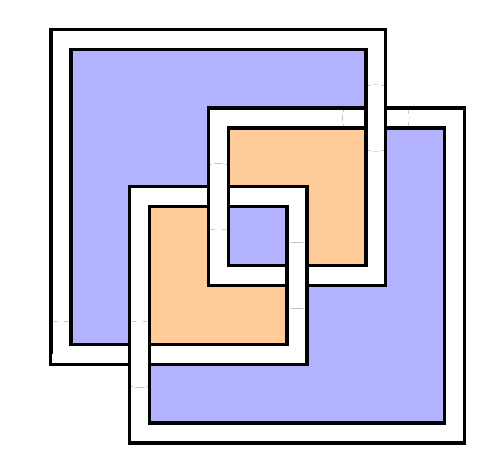
\begin{tikzpicture}
    \filldraw[fill=blue!30] (0, -4)--(0,0)--(4, 0)--(4, -1)--(2, -1)--(2, -2)--(1, -2)--(1, -4)--(0, -4);
    \filldraw[fill=orange!40] (4, -1)--(2, -1)--(2, -2)--(3, -2)--(3, -3)--(4, -3)--(4, -1);
    \filldraw[fill=orange!40] (1, -4)--(3, -4)--(3, -3)--(2, -3)--(2, -2)--(1, -2)--(1, -4);
    \filldraw[fill=blue!30] (2, -3)--(3, -3)--(3, -2)--(2, -2)--(2, -3);
    \filldraw[fill=blue!30] (1, -4)--(1, -5)--(5, -5)--(5, -1)--(4, -1)--(4, -3)--(3, -3)--(3, -3)--(3, -4)--(1, -4);
    \begin{knot}[ 
      consider self intersections,
      ignore endpoint intersections=false,
      clip width=2,
      % draft mode=crossings,
      background color=white,
      only when rendering/.style={
        draw=black,
        double=white,
        double distance=6pt, 
        %line cap=round
      },
      flip crossing=2,
      %flip crossing=5,
      flip crossing=4
      ]
      \strand[very thick] 
        (0, -4) to 
        (0, 0) to 
        (4, 0) to 
        (4, -3) to 
        (2, -3) to 
        (2, -1) to 
        (4, -1) to 
        (5, -1) to 
        (5, -5) to 
        (1, -5) to 
        (1, -2) to 
        (3, -2) to 
        (3, -4) to 
        (0, -4);
    \end{knot}
    \fill[white] (-0.1, -4.09) rectangle (0.18, -3.9);
    \draw[very thick](-0.13, -4)--(-0.13, -4.13)--(0.1, -4.13);


  \end{tikzpicture}

  Przykład kolorowania obszarów węzła.
\end{center}

\begin{definition}{Kolorowanie węzła}{}
  Ponumerujmy łuczki/segmenty węzła, czyli kawałki okręgu między dwoma kolejnymi skrzyżowaniami - będą one $l_1,..., l_n$. Zróbmy to samo ze skrzyżowaniami, które będziemy nazywać $x_1,..., x_n$ i będziemy je traktować jako maszynki, które przyjmują kolory $3$ łuczków: \textbf{górny, wchodzący i wychodzący}, i mówią, czy kolorowanie jest dobre (wartość $0$) czy nie (wartość różna od $0$).

  {\bfseries\color{green}Kolorowaniem nazwiemy przyporządkowanie łuczkom kolorów (liczb całkowitych). Kolorowanie jest sensowne, jeśli przyporządkujemy w taki sposób, że każde skrzyżowanie zwraca nam liczbę $\boldsymbol0$.}
\end{definition}

Każdy artysta ma inną paletę, więc maszynki którymi są skrzyżowania mogą działać na wiele sposobów. My dzisiaj będziemy się zajmować dwoma konkretnymi paletami, które działają jak funkcje:
\begin{align*}
  x_i^+(u, i, o)=(1-t)u+ti-o \quad & \quad x_i^-(u,i,o)=(1-t^{-1})u+t^{-1}i-o\\ 
  x_i^+(u,i,o)=2u-i-o \quad & \quad x_i^-(u,i,o)=2u-i-o
\end{align*}
Zauważmy, że dolny wiersz powstał z górnego przez podstawienie $t\mapsto -1$.

Zaczniemy od działania na drugiej palecie z racji, że jest prostsza. Możemy ją zapisać w postaci \emph{macierzy}, chociaż nie kwadratowej:
$$\begin{bmatrix}2&-1&-1\end{bmatrix}\begin{bmatrix}u\\i\\o\end{bmatrix}$$
Mając kilka skrzyżowań możemy zbudować z takich poziomych paseczków większą, kwadratową macierz, którą będziemy nakładać na kolumn zawierające interesujące nas kolory łuczków. Lepiej pokazać to na przykładzie.

\begin{center}
  \begin{tikzpicture}
    \begin{knot}[
      consider self intersections, 
      clip width = 20pt, 
      % draft mode=crossings, 
      flip crossing=2
      ] 
      \strand[->, thick] (90:2) to[out=0, in=-60, looseness=2]
      (210:2) to[out=120, in=60, looseness=2]
      (-30:2) to[out=-120, in=180, looseness=2] 
      (90:2);
    \end{knot}

    \node at (90:2.5) {$l_1$};
    \node at (210:2.5) {$l_2$};
    \node at (-30:2.5) {$l_3$};

    \node at (150:2) {$x_3$};
    \node at (30:2) {$x_1$};
    \node at (-90:2) {$x_2$};

    \begin{scope}[shift={(6, 0)}]
      \matrix (m) [
        matrix of nodes, 
        left delimiter = {[}, 
        right delimiter={]},
        column sep=5mm
      ]
        {
                2  & -1 & -1  \\
                -1 & -1  & 2  \\
                -1  & 2  & -1 \\
        };
        \node at ($(m-1-1)+(0, .6)$) {$l_1$};
        \node at ($(m-1-2)+(0, .6)$) {$l_2$};
        \node at ($(m-1-3)+(0, .6)$) {$l_3$};

        \node at ($(m-1-1)+(-1, 0)$) {$x_1$};
        \node at ($(m-2-1)+(-1, 0)$) {$x_2$};
        \node at ($(m-3-1)+(-1, 0)$) {$x_3$};
    \end{scope}
  \end{tikzpicture}
\end{center}

Spróbujmy policzyć to samo, ale dla troszkę innego diagramu tego węzła, np. po pierwszym ruchu Reidemeistera na $l_1$.

Mamy dwie macierze, jak będzie czas to można poprosić uczestników o poszukanie niezmienników? (mam nadzieje, że strzelą w wyznacznik, bo on w tym momencie jest zawsze $0$).

Wyznacznik macierzy jaką w ten sposób dostajemy zawsze jest $0$, niezależnie od tego, jaki węzeł kolorujemy. Wynika to z faktu, że zawsze każdy węzeł możemy pokolorować "każdy łuczek jest czerwony". Wystarczy zauważyć, że współczynniki palety sumują się do $0$. Żeby więc dostać wiadomość unikalną dla rozważanego węzła, potrzebujemy usunąć informację o jednym kolorowaniu. Najłatwiej jest to zrobić usuwając jedną kolumnę, ale wtedy mamy macierz niekwadratową - nie umiemy wyliczyć jej wyznacznika. Musimy więc usunąć jeszcze wiersz - można się przekonać, że $\pm1$ zawsze dostajemy to samo, nieważne który wiersz wyrzucimy (nad $\Z[t, t^{-1}]$ to jest $\pm t^{k}$ dla $k\in\Z$). 

Dlaczego usunięcie kolumny działa? Bo odwzorowanie nie jest różnowartościowe - dla każdego $x\in\Z$ mamy $(x,...,x)\mapsto (0,...,0)$. Co prawda to bardziej jest dla przestrzeni wektorowych, ale nie mam ochoty wchodzić w formalności tutaj.

\section{Dlaczego kolorowanie jest niezmiennikiem?}

Szybko na wiarę mówimy, że jeśli macierz zmienimy tak, aby cały lewy dolny trójkąt był $0$, to wtedy wyznacznik możemy szybko liczyć mnożąc wszystkie elementy na przekątnej. Troszkę rzeczy tutaj zamiatam, ale jesteśmy w tęczowej krainie PIDów i się cieszymy.

Rysujemy ruchy Reidemeistera jeszcze raz i pokazujemy co one zmieniają w macierzach
\begin{center}
  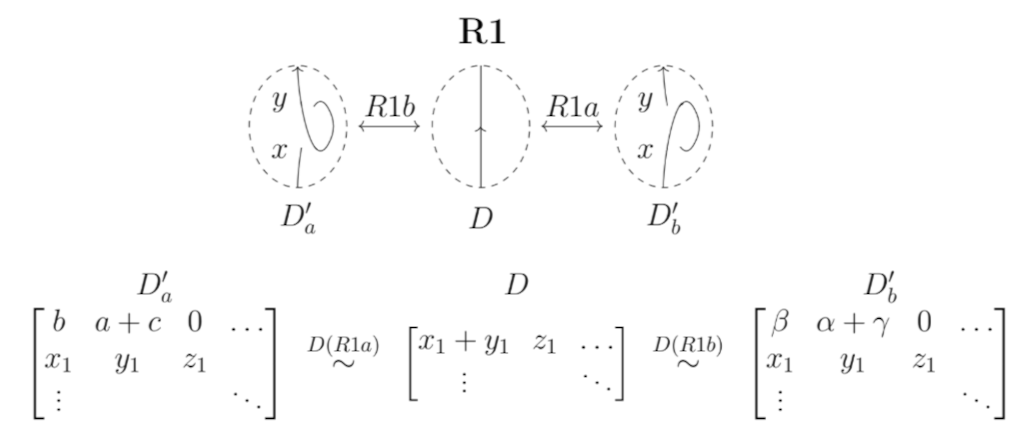
\includegraphics[width=15cm]{R1_matrices.png}

  Tutaj przykład jednego ruchu, reszta idzie podobnie. Palety były nieco ogólniejsze, bo odpowiednio $au+bi+co$ oraz $\alpha u+\beta i+\gamma o$.
\end{center}

Przedstawiam operacje kolumnowe i wierszowe (zmiana kolejności, dodawanie kombinacji liniowej kolumn/wierszy do innej kolumny/wiersza) i pokazuję, że drugi ruch Reidemeistera nie zmienia rzeczy na przekątnej z dokładnością do $\pm1$. Jako zadanie zostawiam ruch pierwszy, a trzeci zostawiam jako dla odważnych (bo jest dłuższy).

\section{Zadania}

Jako zadania chcę dać kilka węzłów, ale np. dwa mają ten sam wielomian Alexandera ($6_1$ i $9_{46}$) a trzy pozostałe mają różny wielomian (nawet po podstawieniu $t\mapsto -1$). Łatwo jest podzielić węzły na $4$ grupki, ale te dwa z tym samym wielomianem są trudniejsze. Jeśli zostanie czasu, to opowiem o tym, że czasem na przekątnej dostajemy tylko jednostki i jedną nie-jednostkę, a czasem zdarzają się dwie nie-jednostki (Smith normal form). To też jest przydatne do rozróżniania węzłów (nie zawsze co prawda, ale działa dla przykładu z 6 i 9 skrzyżowaniami) c:


\end{document}
